\documentclass{standalone}
\usepackage[utf8]{inputenc}
\usepackage{csvsimple}
\usepackage{tikz}
\usetikzlibrary{plotmarks}
\usepackage{pgfplots}
\usepackage{pgfplotstable}
\usepackage{filecontents}
\usetikzlibrary{backgrounds}
\pgfplotsset{compat=newest}
\usetikzlibrary{arrows}
\usepackage{relsize}
\usepackage{filecontents}
\usetikzlibrary{hobby}
\usetikzlibrary{arrows}
\tikzset{fontscale/.style = {font=\relsize{#1}}
	}

\begin{document}
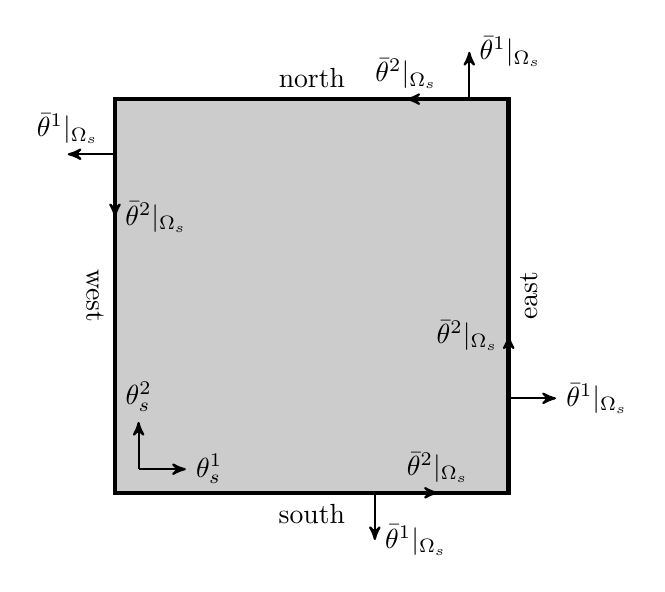
\begin{tikzpicture}[scale = 1, use Hobby shortcut,axis/.style={thick,  ->, >=stealth'}]
	\filldraw[fill=gray!40!white, draw=black, ultra thick] (0,0) -- node[sloped,midway,below] {south} (5,0) -- node[sloped,midway,below] {east}  (5, 5) --node[sloped,midway,above] {north}  (0, 5) -- node[sloped,midway,below] {west}  cycle;

	\begin{scope}[shift={(.3,.3)}]
		\draw[axis] (0,0)  -- (.6,0) node[right]
		{$\theta^1_s$};
		\draw[axis] (0,0)  -- (0,.6) node[above]
        {$\theta^2_s$};
	\end{scope}

	\begin{scope}[shift={(3.3,0)}, rotate=-90]
		\draw[axis] (0,0)  -- (.6,0) node[right]
		{$\bar{\theta}^1\vert_{\Omega_s}$};
		\draw[axis] (0,0)  -- (0,.8) node[above]
        {$\bar{\theta}^2\vert_{\Omega_s}$};
	\end{scope}

	\begin{scope}[shift={(5,1.2)}, rotate=-0]
		\draw[axis] (0,0)  -- (.6,0) node[right]
		{$\bar{\theta}^1\vert_{\Omega_s}$};
		\draw[axis] (0,0)  -- (0,.8) node[left]
        {$\bar{\theta}^2\vert_{\Omega_s}$};
	\end{scope}

	\begin{scope}[shift={(4.5,5)}, rotate=90]
		\draw[axis] (0,0)  -- (.6,0) node[right]
		{$\bar{\theta}^1\vert_{\Omega_s}$};
		\draw[axis] (0,0)  -- (0,.8) node[above]
        {$\bar{\theta}^2\vert_{\Omega_s}$};
	\end{scope}

	\begin{scope}[shift={(0,4.3)}, rotate=-180]
		\draw[axis] (0,0)  -- (.6,0) node[above]
		{$\bar{\theta}^1\vert_{\Omega_s}$};
		\draw[axis] (0,0)  -- (0,.8) node[right]
        {$\bar{\theta}^2\vert_{\Omega_s}$};
	\end{scope}
\end{tikzpicture}
\end{document}